%package list
\documentclass{article}
\usepackage[top=3cm, bottom=3cm, outer=3cm, inner=3cm]{geometry}
\usepackage{multicol}
\usepackage{graphicx}
\usepackage{url}
%\usepackage{cite}
\usepackage{hyperref}
\usepackage{array}
%\usepackage{multicol}
\newcolumntype{x}[1]{>{\centering\arraybackslash\hspace{0pt}}p{#1}}
\usepackage{natbib}
\usepackage{pdfpages}
\usepackage{multirow}
\usepackage[normalem]{ulem}
\useunder{\uline}{\ul}{}
\usepackage{svg}
\usepackage{xcolor}
\usepackage{listings}
\lstdefinestyle{ascii-tree}{
    literate={├}{|}1 {─}{--}1 {└}{+}1 
  }
\lstset{basicstyle=\ttfamily,
  showstringspaces=false,
  commentstyle=\color{red},
  keywordstyle=\color{blue}
}
%\usepackage{booktabs}
\usepackage{caption}
\usepackage{subcaption}
\usepackage{float}
\usepackage{array}

\newcolumntype{M}[1]{>{\centering\arraybackslash}m{#1}}
\newcolumntype{N}{@{}m{0pt}@{}}


%%%%%%%%%%%%%%%%%%%%%%%%%%%%%%%%%%%%%%%%%%%%%%%%%%%%%%%%%%%%%%%%%%%%%%%%%%%%
%%%%%%%%%%%%%%%%%%%%%%%%%%%%%%%%%%%%%%%%%%%%%%%%%%%%%%%%%%%%%%%%%%%%%%%%%%%%
\newcommand{\itemEmail}{}
\newcommand{\itemStudent}{Andre David Delgado Allpan,\newline Andre Hilacondo Begazo,\newline Gonzalo  Layme Mamani,\newline  Diego Llerena Tellez,\newline  Mauricio Zegarra Puma}
\newcommand{\itemCourse}{Estructura de datos y algoritmos}
\newcommand{\itemCourseCode}{20231001}
\newcommand{\itemSemester}{III}
\newcommand{\itemUniversity}{Universidad Nacional de San Agustín de Arequipa}
\newcommand{\itemFaculty}{Facultad de Ingeniería de Producción y Servicios}
\newcommand{\itemDepartment}{Departamento Académico de Ingeniería de Sistemas e Informática}
\newcommand{\itemSchool}{Escuela Profesional de Ingeniería de Sistemas}
\newcommand{\itemAcademic}{2023 - A}
\newcommand{\itemInput}{Del 10 Julio 2023}
\newcommand{\itemOutput}{Al 17 Julio 2023}
\newcommand{\itemPracticeNumber}{06}
\newcommand{\itemTheme}{Tries}
%%%%%%%%%%%%%%%%%%%%%%%%%%%%%%%%%%%%%%%%%%%%%%%%%%%%%%%%%%%%%%%%%%%%%%%%%%%%
%%%%%%%%%%%%%%%%%%%%%%%%%%%%%%%%%%%%%%%%%%%%%%%%%%%%%%%%%%%%%%%%%%%%%%%%%%%%

\usepackage[english,spanish]{babel}
\usepackage[utf8]{inputenc}
\AtBeginDocument{\selectlanguage{spanish}}
\renewcommand{\figurename}{Figura}
\renewcommand{\refname}{Referencias}
\renewcommand{\tablename}{Tabla} %esto no funciona cuando se usa babel
\AtBeginDocument{%
	\renewcommand\tablename{Tabla}
}

\usepackage{fancyhdr}
\pagestyle{fancy}
\fancyhf{}
\setlength{\headheight}{30pt}
\renewcommand{\headrulewidth}{1pt}
\renewcommand{\footrulewidth}{1pt}
\fancyhead[L]{\raisebox{-0.2\height}{
\includegraphics[width=3cm]{img/logo_episunsa.png}}}
\fancyhead[C]{\fontsize{7}{7}\selectfont	\itemUniversity \\ \itemFaculty \\ \itemDepartment \\ \itemSchool \\ \textbf{\itemCourse}}
\fancyhead[R]{\raisebox{-0.2\height}{
\includegraphics[width=1.2cm]{img/logo_abet}}}
\fancyfoot[L]{Prof. Edith Cano }
\fancyfoot[C]{\itemCourse}
\fancyfoot[R]{Página \thepage}

% para el codigo fuente
\usepackage{listings}
\usepackage{color, colortbl}
\definecolor{dkgreen}{rgb}{0,0.6,0}
\definecolor{gray}{rgb}{0.5,0.5,0.5}
\definecolor{mauve}{rgb}{0.58,0,0.82}
\definecolor{codebackground}{rgb}{0.95, 0.95, 0.92}
\definecolor{tablebackground}{rgb}{0.8, 0, 0}

\lstset{frame=tb,
	language=bash,
	aboveskip=3mm,
	belowskip=3mm,
	showstringspaces=false,
	columns=flexible,
	basicstyle={\small\ttfamily},
	numbers=none,
	numberstyle=\tiny\color{gray},
	keywordstyle=\color{blue},
	commentstyle=\color{dkgreen},
	stringstyle=\color{mauve},
	breaklines=true,
	breakatwhitespace=true,
	tabsize=3,
	backgroundcolor= \color{codebackground},
}

\begin{document}
	
	\vspace*{10px}
	
	\begin{center}	
		\fontsize{17}{17} \textbf{ Informe de Laboratorio \itemPracticeNumber}
	\end{center}
	\centerline{\textbf{\Large Tema: \itemTheme}}
	%\vspace*{0.5cm}	

	\begin{flushright}
		\begin{tabular}{|M{2.5cm}|N|}
			\hline 
			\rowcolor{tablebackground}
			\color{white} \textbf{Nota}  \\
			\hline 
			     \\[30pt]
			\hline 			
		\end{tabular}
	\end{flushright}	

	\begin{table}[H]
		\begin{tabular}{|x{4.7cm}|x{4.8cm}|x{4.8cm}|}
			\hline 
			\rowcolor{tablebackground}
			\color{white} \textbf{Estudiantes} & \color{white}\textbf{Escuela}  & \color{white}\textbf{Asignatura}   \\
			\hline 
			{\itemStudent \par \itemEmail} & \itemSchool & {\itemCourse \par Semestre: \itemSemester \par Código: \itemCourseCode}     \\
			\hline 			
		\end{tabular}
	\end{table}		
	
	\begin{table}[H]
		\begin{tabular}{|x{4.7cm}|x{4.8cm}|x{4.8cm}|}
			\hline 
			\rowcolor{tablebackground}
			\color{white}\textbf{Laboratorio} & \color{white}\textbf{Tema}  & \color{white}\textbf{Duración}   \\
			\hline 
			\itemPracticeNumber & \itemTheme & 04 horas   \\
			\hline 
		\end{tabular}
	\end{table}
	
	\begin{table}[H]
		\begin{tabular}{|x{4.7cm}|x{4.8cm}|x{4.8cm}|}
			\hline 
			\rowcolor{tablebackground}
			\color{white}\textbf{Semestre académico} & \color{white}\textbf{Fecha de inicio}  & \color{white}\textbf{Fecha de entrega}   \\
			\hline 
			\itemAcademic & \itemInput &  \itemOutput  \\
			\hline 
		\end{tabular}
	\end{table}
	\section{URL de Repositorio Github}
	\begin{itemize}
		
		\item URL para el laboratorio 06 en el Repositorio GitHub.
		\item \url{https://github.com/GonzaloRail/Laboratorio_06_EDA.git}
	\end{itemize}
	
	
	\section{Tarea}
	\subsection{Introducción}
	\begin{itemize}
		\item En este informe, describiremos la implementación de una Trie con una interfaz gráfica de usuario para permitir al usuario insertar, buscar y reemplazar palabras en un texto. Una Trie es una estructura de datos eficiente para almacenar y buscar palabras o cadenas de caracteres, especialmente cuando hay muchas palabras con prefijos comunes.
	\end{itemize}
	\subsection{Descripción del Trie}
	\begin{itemize}
		\item La Trie se implementa utilizando una estructura de árbol, donde cada nodo del árbol representa un carácter en una palabra. Cada nodo tiene un arreglo de 26 referencias a otros nodos, correspondientes a las 26 letras del alfabeto inglés. Si una palabra tiene un carácter específico en una posición, el nodo correspondiente tendrá una referencia no nula al siguiente nodo que representa la siguiente letra en la palabra.
	\end{itemize}
	\subsection{Métodos principales de la clase Trie}
	\begin{itemize}
		\item insert(String word): Inserta una palabra en la Trie. Comienza desde la raíz y recorre los nodos correspondientes a cada letra de la palabra. Marca el último nodo como el final de la palabra.
		\lstinputlisting[language=Java, 		caption={Trie.java (Metodo insert)},numbers=left,firstline=25, lastline=39]{final/Trie.java}
		
		\item search(String word): Busca una palabra en la Trie. Comienza desde la raíz y recorre los nodos correspondientes a cada letra de la palabra. Si encuentra todos los nodos correspondientes y el último nodo está marcado como el final de una palabra, significa que la palabra está presente en la Trie.
		\lstinputlisting[language=Java, 		caption={Trie.java (Metodo search)},numbers=left,firstline=41, lastline=55]{final/Trie.java}
		\clearpage
		\item delete(String word): Elimina una palabra de la Trie. Comienza desde la raíz y recorre los nodos correspondientes a cada letra de la palabra. Marca el último nodo como no el final de la palabra.
		\lstinputlisting[language=Java, 		caption={Trie.java (Metodo delete)},numbers=left,firstline=76, lastline=90]{final/Trie.java}
		
		\item replace(String word, String replacement): Reemplaza una palabra en la Trie con otra palabra proporcionada. Primero, busca la palabra original y la reemplaza con la nueva palabra. Si la palabra original no está presente, se lanza una excepción.
		\lstinputlisting[language=Java, 		caption={Trie.java (Metodo replace)},numbers=left,firstline=57, lastline=74]{final/Trie.java}
	\end{itemize}
	\clearpage
	
	\clearpage
	\subsection{Estructura de la implementación}
	\begin{itemize}
		\item Trie: La clase principal que representa la Trie y contiene los métodos para insertar, buscar y eliminar palabras.
		\lstinputlisting[language=Java, 		caption={Trie.java},numbers=left,]{final/Trie.java}
	\item TrieNode: Una clase interna de Trie que representa un nodo en la Trie, que contiene las referencias a otros nodos y un indicador para marcar el final de una palabra.
	\lstinputlisting[language=Java, 		caption={Trie.java (Líneas 11-19)},numbers=left,firstline=11, lastline=19]{final/Trie.java}
	
	
	\item TrieGUI: La clase que crea la interfaz gráfica de usuario para interactuar con la Trie.
	\lstinputlisting[language=Java, 		caption={TrieGUI.java },numbers=left]{final/TrieGUI.java}
	
	\end{itemize}
	
	\subsection{Descripcióm general de la clase TrieGUI}
	La clase TrieGUI crea una interfaz gráfica para permitir al usuario interactuar con la Trie. 		    La interfaz gráfica contiene los siguientes componentes:
	\begin{itemize}
		\item Etiquetas: Etiquetas para indicar qué acción realizar (insertar, buscar, reemplazar).
		\item Botones: Botones para realizar las acciones de inserción, búsqueda y reemplazo.
		\item Cuadros de texto: Campos de texto para ingresar palabras y ver la salida en la consola y el contenido actual en la Trie.
		
		\begin{figure}[H]
		\centering
		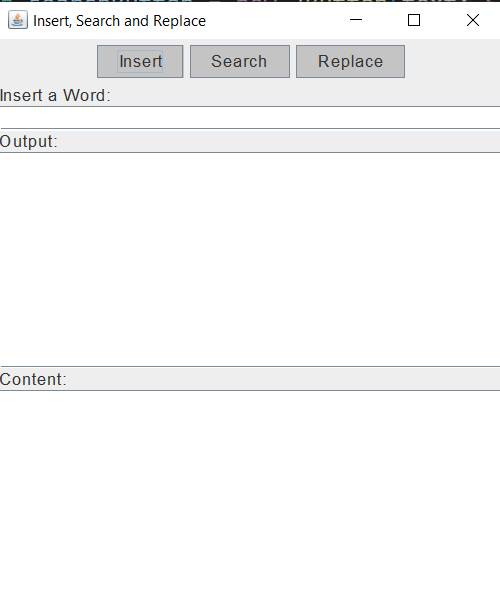
\includegraphics[width=0.7\textwidth, 		height=0.7\textwidth,keepaspectratio]{pruebas/visual1.png}
	\end{figure}

	\end{itemize}
	\clearpage
	\subsection{Descripcióm general de la clase TrieGUI}
	La clase TrieGUI crea una interfaz gráfica para permitir al usuario interactuar con la Trie. 		    La interfaz gráfica contiene los siguientes componentes:
	\begin{itemize}
		\item Etiquetas: Etiquetas para indicar qué acción realizar (insertar, buscar, reemplazar).
		\item Botones: Botones para realizar las acciones de inserción, búsqueda y reemplazo.
		\item Cuadros de texto: Campos de texto para ingresar palabras y ver la salida en la consola y el contenido actual en la Trie.
		
		\begin{figure}[H]
		\centering
		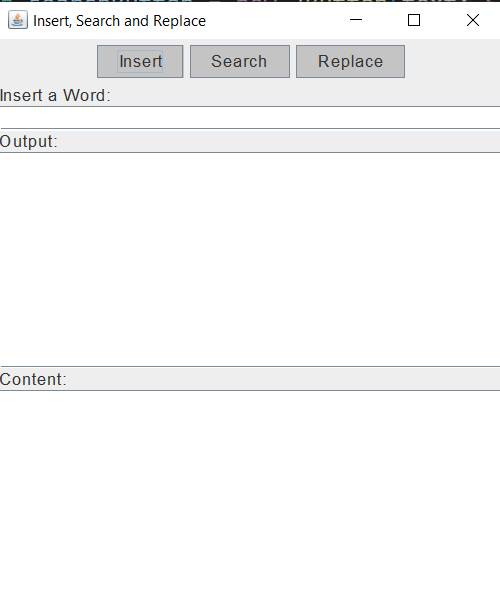
\includegraphics[width=0.7\textwidth, height=0.7\textwidth,keepaspectratio]{pruebas/visual1.png}
	\end{figure}
	
	\end{itemize}
	\clearpage
	\subsection{Funcionamiento de la aplicación}
	
	\begin{itemize}
		\item Al ejecutar la aplicación, se mostrará una ventana con la interfaz gráfica.
		\begin{figure}[H]
		\centering
		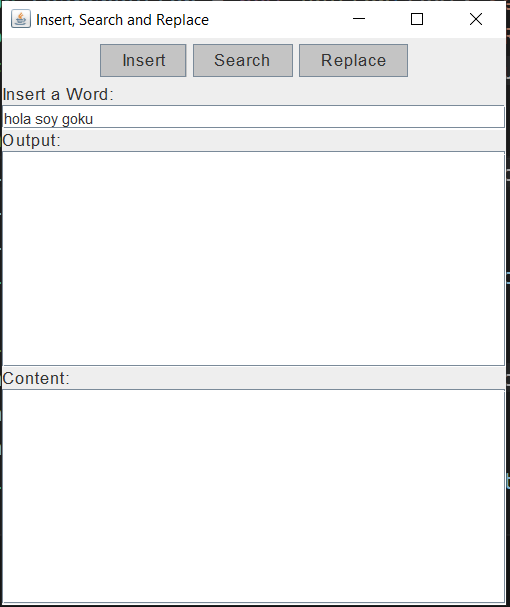
\includegraphics[width=0.7\textwidth, height=0.7\textwidth,keepaspectratio]{pruebas/visual2.png}
		\end{figure}
		\clearpage
		
		\item El usuario puede ingresar una palabra en el campo de texto y luego hacer clic en el botón "Insert" para insertar la palabra en la Trie.
		
		\begin{figure}[H]
		\centering
		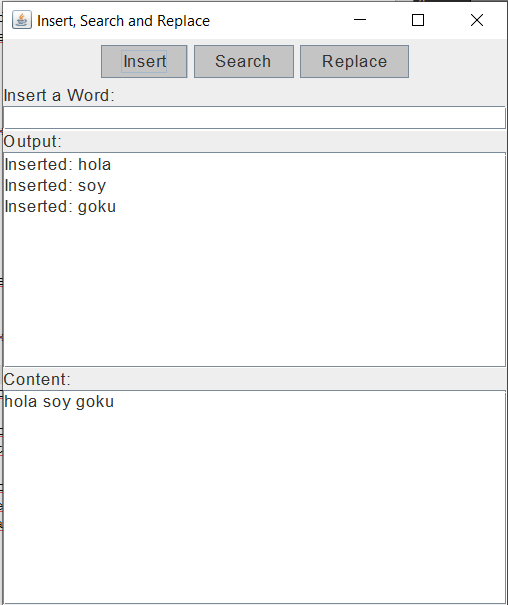
\includegraphics[width=0.7\textwidth, height=0.7\textwidth,keepaspectratio]{pruebas/insert.png}
		\end{figure}
		\clearpage
		\item El usuario puede ingresar una palabra en el campo de texto y luego hacer clic en el botón "Search" para buscar la palabra en la Trie. El resultado de la búsqueda se mostrará en la consola.
		\begin{figure}[H]
		\centering
		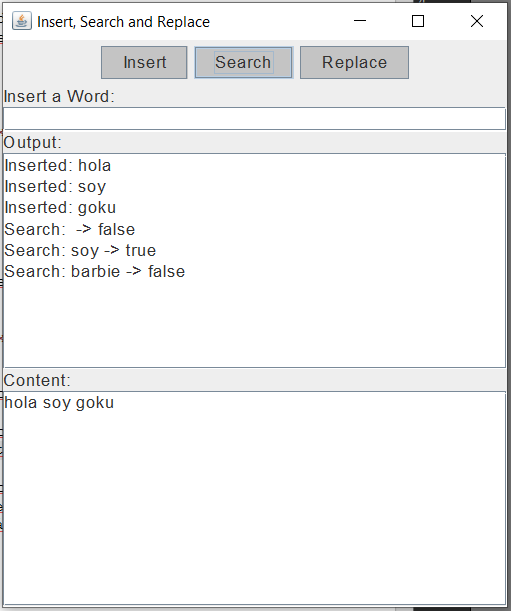
\includegraphics[width=0.7\textwidth, height=0.7\textwidth,keepaspectratio]{pruebas/search.png}
		\end{figure}
		\clearpage
		\item El usuario puede ingresar una palabra en el campo de texto y luego hacer clic en el botón "Replace". Se le pedirá que ingrese una palabra de reemplazo. La aplicación reemplazará la palabra original con la nueva palabra en la Trie y mostrará el resultado actualizado en la consola y el contenido actual en la Trie.
		\begin{figure}[H]
		\centering
		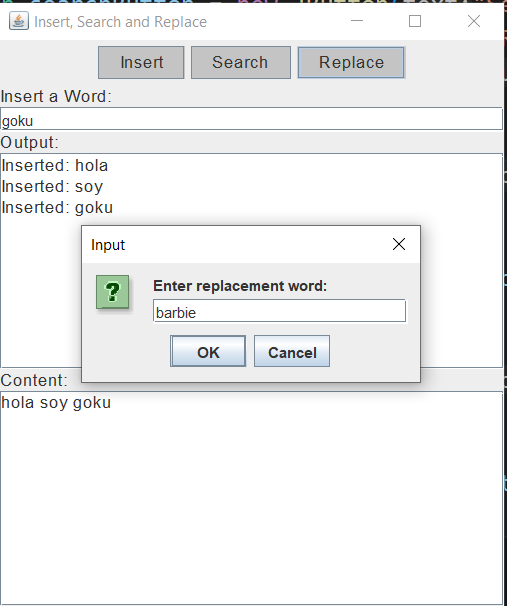
\includegraphics[width=0.5\textwidth, height=0.5\textwidth,keepaspectratio]{pruebas/replace1.png}
		\end{figure}
		\begin{figure}[H]
		\centering
		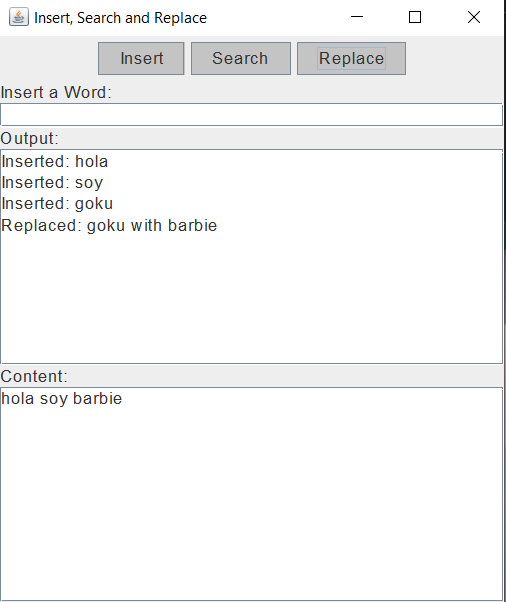
\includegraphics[width=0.5\textwidth, height=0.5\textwidth,keepaspectratio]{pruebas/replace2.png}
		\end{figure}
		\clearpage
		

	\end{itemize}
	\subsection{Conclusiones}
	\begin{itemize}
		\item En la tarea de implementar un Trie con interfaz gráfica de usuario para insertar, buscar y reemplazar palabras en un texto, hemos visto que los Trie son una estructura de datos altamente eficiente para manejar y manipular un conjunto grande de palabras, especialmente cuando existen prefijos comunes entre ellas.

		\item Los Trie nos permiten realizar búsquedas de palabras en tiempo lineal en función del tamaño de la palabra y no del tamaño total del conjunto de palabras. Esto los convierte en una excelente opción para implementar aplicaciones como correctores ortográficos, autocompletado de palabras y sistemas de sugerencias de búsqueda, donde la búsqueda rápida y eficiente es esencial.
	\end{itemize}
	\section{Cuestionario}
\begin{itemize}
	\item \textbf{Explique. ¿Cómo se utiliza esta estructura de datos para almacenar prefijos?} \\
		En un Trie, cada nodo representa un carácter y cada camino desde la raíz hasta un nodo hoja representa una palabra completa. La idea clave detrás del Trie es que los nodos comparten los mismos prefijos comunes. Esto significa que las palabras que comparten un prefijo comparten nodos en común en el Trie. 
		Utilizando una clase Trie y una clase interna TrieNode. La clase TrieNode representa un nodo en el Trie y contiene un arreglo de referencias a otros nodos, correspondientes a las 26 letras del alfabeto inglés. Cada nodo también tiene un indicador booleano isWord, que marca si el nodo representa el final de una palabra.

Cuando se inserta una palabra en el Trie utilizando el método insert(String word), el algoritmo recorre los caracteres de la palabra y crea nuevos nodos si no existen para representar cada carácter. Esto asegura que se construya un camino desde la raíz hasta el nodo que representa el último carácter de la palabra, formando así la palabra completa.

El uso de la estructura Trie para almacenar prefijos permite que las búsquedas de palabras y la comprobación de existencia de palabras sean rápidas. Dado que los prefijos comunes se comparten entre las palabras, la búsqueda puede detenerse cuando se alcanza un punto en el Trie donde ya no hay más caracteres que coincidan con el prefijo buscado.
	\item \textbf{Cómo realizó la funcionalidad de reemplazar texto} \\
	La funcionalidad de reemplazar texto se ha implementado en el método replace(String word, String replacement) de la clase Trie. El objetivo es reemplazar una palabra word existente en el Trie con una nueva palabra replacement.

El método replace se divide en tres partes:

    Primero, busca la palabra word en el Trie utilizando el algoritmo de búsqueda similar al utilizado en el método search(String word). Si encuentra la palabra, procede a la siguiente etapa. Si no encuentra la palabra, se lanza una excepción.

    Luego, se recorre la lista content, que contiene todas las palabras previamente insertadas en el Trie. Si encuentra la palabra word en la lista content, la reemplaza con la nueva palabra replacement.

    Después de actualizar la lista content, el método elimina la palabra word del Trie utilizando el método delete(String word), asegurándose de que el nodo correspondiente al último carácter de la palabra tenga isWord establecido en false. Luego, inserta la nueva palabra replacement en el Trie utilizando el método insert(String word), creando un nuevo camino para la palabra reemplazada.
\end{itemize}
	\clearpage
	
	
	\section{\textcolor{red}{Rúbricas}}
	
	\subsection{\textcolor{red}{Entregable Informe}}
	\begin{table}[H]
		\caption{Tipo de Informe}
		\setlength{\tabcolsep}{0.5em} % for the horizontal padding
		{\renewcommand{\arraystretch}{1.5}% for the vertical padding
		\begin{tabular}{|p{3cm}|p{12cm}|}
			\hline
			\multicolumn{2}{|c|}{\textbf{\textcolor{red}{Informe}}}  \\
			\hline 
			\textbf{\textcolor{red}{Latex}} & \textcolor{blue}{El informe está en formato PDF desde Latex,  con un formato limpio (buena presentación) y facil de leer.}   \\ 
			\hline 
			
			
		\end{tabular}
	}
	\end{table}
	
	\clearpage
	
	\subsection{\textcolor{red}{Rúbrica para el contenido del Informe y demostración}}
	\begin{itemize}			
		\item El alumno debe marcar o dejar en blanco en celdas de la columna \textbf{Checklist} si cumplio con el ítem correspondiente.
		\item Si un alumno supera la fecha de entrega,  su calificación será sobre la nota mínima aprobada, siempre y cuando cumpla con todos lo items.
		\item El alumno debe autocalificarse en la columna \textbf{Estudiante} de acuerdo a la siguiente tabla:
	
		\begin{table}[ht]
			\caption{Niveles de desempeño}
			\begin{center}
			\begin{tabular}{ccccc}
    			\hline
    			 & \multicolumn{4}{c}{Nivel}\\
    			\cline{1-5}
    			\textbf{Puntos} & Insatisfactorio 25\%& En Proceso 50\% & Satisfactorio 75\% & Sobresaliente 100\%\\
    			\textbf{2.0}&0.5&1.0&1.5&2.0\\
    			\textbf{4.0}&1.0&2.0&3.0&4.0\\
    		\hline
			\end{tabular}
		\end{center}
	\end{table}	
	
	\end{itemize}
	
	\begin{table}[H]
		\caption{Rúbrica para contenido del Informe y demostración}
		\setlength{\tabcolsep}{0.5em} % for the horizontal padding
		{\renewcommand{\arraystretch}{1.5}% for the vertical padding
		%\begin{center}
		\begin{tabular}{|p{2.7cm}|p{7cm}|x{1.3cm}|p{1.2cm}|p{1.5cm}|p{1.1cm}|}
			\hline
    		\multicolumn{2}{|c|}{Contenido y demostración} & Puntos & Checklist & Estudiante & Profesor\\
			\hline
			\textbf{1. GitHub} & Hay enlace URL activo del directorio para el  laboratorio hacia su repositorio GitHub con código fuente terminado y fácil de revisar. &2 &X &2 & \\ 
			\hline
			\textbf{2. Commits} &  Hay capturas de pantalla de los commits más importantes con sus explicaciones detalladas. (El profesor puede preguntar para refrendar calificación). &4 & & & \\ 
			\hline 
			\textbf{3. Código fuente} &  Hay porciones de código fuente importantes con numeración y explicaciones detalladas de sus funciones. &2 &X &2 & \\ 
			\hline 
			\textbf{4. Ejecución} & Se incluyen ejecuciones/pruebas del código fuente  explicadas gradualmente. &2 &X &2 & \\ 
			\hline			
			\textbf{5. Pregunta} & Se responde con completitud a la pregunta formulada en la tarea.  (El profesor puede preguntar para refrendar calificación).  &2 &X &2 & \\ 
			\hline	
			\textbf{6. Fechas} & Las fechas de modificación del código fuente estan dentro de los plazos de fecha de entrega establecidos. &2 &X &2 & \\ 
			\hline 
			\textbf{7. Ortografía} & El documento no muestra errores ortográficos. &2 &X &2 & \\ 
			\hline 
			\textbf{8. Madurez} & El Informe muestra de manera general una evolución de la madurez del código fuente,  explicaciones puntuales pero precisas y un acabado impecable.   (El profesor puede preguntar para refrendar calificación).  &4 & & & \\ 
			\hline
			\multicolumn{2}{|c|}{\textbf{Total}} &20 & &12 & \\ 
			\hline
		\end{tabular}
		%\end{center}
		%\label{tab:multicol}
		}
	\end{table}
	
\clearpage

\section{Referencias}
\begin{itemize}			
	\item \url{https://www.w3schools.com/java/default.asp}
	\item \url{https://www.geeksforgeeks.org/insertion-sort/}
\end{itemize}	
	
%\clearpage
%\bibliographystyle{apalike}
%\bibliographystyle{IEEEtranN}
%\bibliography{bibliography}
			
\end{document}